\section{Experimental Task Details}\label{appendix:tasks}

\begin{table}[!h]
    \caption{Task specific hyperparameters, see introduction for definitions.}
    \label{table:hyperparams}
    \begin{center}
        \begin{tabular}{l | l l l l l l}
            \toprule
            {\bf Task} & \textbf{Training Steps} & \textbf{Warmup} & \textbf{Seq. Length} & $E$ & $A$ & $M$ \\
            \midrule
            IMDb Token Level & $30k$ & $8k$ & $1k$ & 512 & 64 & 2048 \\
            IMDb Byte Level & $30k$ & $8k$ & $1k$ & 512 & 64 & 2048 \\
            Listops & $10k$ & $1k$ & $2k$ & 512 & 64 & 2048 \\
            Document Matching & $10k$ & $8k$ & $4k$ & 128 & 32 & 512 \\
            \bottomrule
        \end{tabular}
    \end{center}
\end{table}

In all tasks we tested on, we used an Adam optimiser with linear warmup and square root decay.
We used a base learning rate of 0.05, $\beta_1=0.9$, and $\beta_2=0.98$ and a batch size of 32 for every task.
Attention kernel and MLP weights were initialised via uniform xavier.
Biases, input embeddings, and positional embeddings were initialised via Gaussian distributions with variances of $10^{-6}$, $1$, and $0.02$ respectively. 
All attention mechanisms, except Sinkhorn, used the [CLS] token for classification.
Sinkhorn used mean classifier pooling.
Task specific hyperparameters are given in \cref{table:hyperparams}.
In all Transformer models the feed-forward network (FFN) has a single hidden dimension.
Before testing we take the model which had the best validation accuracy during training, the long train times are to ensure convergence.


\section{Model Size}\label{appendix:model_size}

\begin{table}[!h]
    \caption{Model sizes for all tasks and attentions for deepest and widest models (MiB).}
    \label{table:model_sizes}
    \begin{center}
        \begin{tabular}{l | l l l l l l l l | l l}
            \toprule
            {\bf Attention} & \multicolumn{2}{c}{\bf IMDb Token} & \multicolumn{2}{c}{\bf IMDb Byte} & \multicolumn{2}{c}{\bf Listops} & \multicolumn{2}{c}{\bf Doc Matching} & \multicolumn{2}{c}{\bf Average} \\
            {\bf Type} & Deep & Wide & Deep & Wide & Deep & Wide & Deep & Wide & Deep & Wide \\
            \midrule
BigBird     & 779 & 659 & 230 & 110 & 229 & 109 & 13 & 8.0 & 313 & 222 \\
Linear      & 779 & 659 & 230 & 110 & 229 & 109 & 13 & 8.0 & 313 & 222 \\
Linformer   & 780 & 659 & 232 & 110 & 231 & 109 & 16 & 8.7 & 315 & 222 \\
Local       & 779 & 659 & 230 & 110 & 229 & 109 & 13 & 8.0 & 313 & 222 \\
Longformer  & 833 & 713 & 284 & 164 & 283 & 163 & 15 & 11 & 354 & 263 \\
Performer   & 779 & 659 & 230 & 110 & 229 & 109 & 13 & 8.0 & 313 & 222 \\
Sinkhorn    & 767 & 647 & 218 & 98 & 217 & 97 & 13 & 8.0 & 304 & 213 \\
Sparse      & 779 & 659 & 230 & 110 & 229 & 109 & 13 & 8.0 & 313 & 222 \\
Synthesizer & 761 & 641 & 230 & 109 & 300 & 179 & 60 & 55 & 338 & 246 \\
Transformer & 779 & 659 & 230 & 110 & 229 & 109 & 13 & 8.0 & \textbf{313} & \textbf{222}  \\
\bottomrule
Average     & 782 & 661 & 234 & 114 & 241 & 120 & 18 & 13.1 & \textbf{319} & \textbf{227} \\
        \end{tabular}
    \end{center}
\end{table}

\Cref{table:model_sizes} shows the size of the deepest and widest models for every task and attention combination in mebibytes.


\section{Latency}\label{appendix:latency}

\begin{table}[!h]
    \caption{Latency for all tasks and attentions for deepest and widest models on a CPU (ms).}
    \label{table:cpu_latency}
    \begin{center}
        \begin{tabular}{l | l l l l l l l l | l l}
            \toprule
            {\bf Attention} & \multicolumn{2}{c}{\bf IMDb Token} & \multicolumn{2}{c}{\bf IMDb Byte} & \multicolumn{2}{c}{\bf Listops} & \multicolumn{2}{c}{\bf Doc Matching} & \multicolumn{2}{c}{\bf Average} \\
            {\bf Type} & Deep & Wide & Deep & Wide & Deep & Wide & Deep & Wide & Deep & Wide \\
            \midrule
BigBird     & 116 & 46 & 106 & 24 & 103 & 30 & 125 & 33 & 113 & 33 \\
Linear      & 54 & 33 & 33 & 11 & 33 & 11 & 26 & 10 & 37 & 16 \\
Linformer   & 60 & 34 & 39 & 12 & 39 & 12 & 34 & 12 & 43 & 18 \\
Local       & 59 & 34 & 34 & 11 & 33 & 12 & 27 & 11 & 38 & 17 \\
Longformer  & 70 & 37 & 62 & 17 & 149 & 37 & 939 & 263 & 305 & 89 \\
Performer   & 53 & 33 & 32 & 11 & 55 & 35 & 28 & 9 & 42 & 22 \\
Sinkhorn    & 83 & 39 & 59 & 16 & 59 & 17 & 58 & 21 & 65 & 23 \\
Sparse      & 56 & 40 & 38 & 14 & 47 & 27 & 88 & 66 & 57 & 37 \\
Synthesizer & 257 & 237 & 866 & 11 & 130 & 20 & 45 & 23 & 324 & 73 \\
Transformer & 60 & 34 & 40 & 13 & 41 & 16 & 56 & 36 & \textbf{49} & \textbf{25}  \\
\bottomrule
Average     & 87 & 57 & 131 & 14 & 69 & 22 & 140 & 48 & \textbf{107} & \textbf{35} \\
        \end{tabular}
    \end{center}
\end{table}

\begin{table}[!h]
    \caption{Latency for all tasks and attentions for deepest and widest models on a GPU (ms). Averages across attention ignore Synthesizer due to its \emph{extreme} results.}
    \label{table:gpu_latency}
    \begin{center}
        \begin{tabular}{l | l l l l l l l l | l l}
            \toprule
            {\bf Attention} & \multicolumn{2}{c}{\bf IMDb Token} & \multicolumn{2}{c}{\bf IMDb Byte} & \multicolumn{2}{c}{\bf Listops} & \multicolumn{2}{c}{\bf Doc Matching} & \multicolumn{2}{c}{\bf Average} \\
            {\bf Type} & Deep & Wide & Deep & Wide & Deep & Wide & Deep & Wide & Deep & Wide \\
            \midrule
BigBird     & 154          & 63 & 154 & 59 & 210 & 128 & 232  & 115 & 188 & 91 \\
Linear      & 52           & 21 & 63 & 37  & 76  & 32 & 52    & 22 & 61 & 28 \\
Linformer   & 58           & 21 & 73 & 38  & 81  & 32 & 58    & 23 & 68 & 29 \\
Local       & 58           & 26 & 68 & 41  & 86  & 40 & 63    & 34 & 69 & 35 \\
Longformer  & 115          & 57 & 83 & 48  & 340 & 189 & 1202 & 540 & 435 & 209 \\
Performer   & 47           & 17 & 60 & 35  & 95  & 51 & 49    & 19 & 63 & 31 \\
Sinkhorn    & 92           & 33 & 112 & 50 & 121 & 49 & 106   & 52 & 108 & 46 \\
Sparse      & 92           & 55 & 76 & 46  & 229 & 175 & 351  & 346 & 187 & 156 \\
Synthesizer & \emph{25164} & 34 & \emph{5927} & \emph{6001}   & 325 & 199 & 338 & 293 & 7939 & 1632 \\
Transformer & 88           & 50 & 75 & 47  & 208 & 170 & 289  & 289 & \textbf{165} & \textbf{139} \\
\bottomrule
Average     & 76           & 34 & 76 & 40  & 145 & 87  & 240  & 144 & \textbf{144} & \textbf{76} \\
        \end{tabular}
    \end{center}
\end{table}

To test latency we input a random full length input into the model 100 times and take the average of the time taken.
The latency times for single input on CPU are given in \Cref{table:cpu_latency}, the hardware used is $2\times$ AMD EPYC 7763 64-Core Processor 1.8GHz.
GPU times are given in \Cref{table:gpu_latency}, for this we input a batch of 32 inputs.
We use a single Nvidia A100-SXM-80GB GPU.


\section{Full attention scores}\label{appendix:attention}

\begin{figure}[!h]
    \centering
    \begin{subfigure}{.35\textwidth}
        \centering
        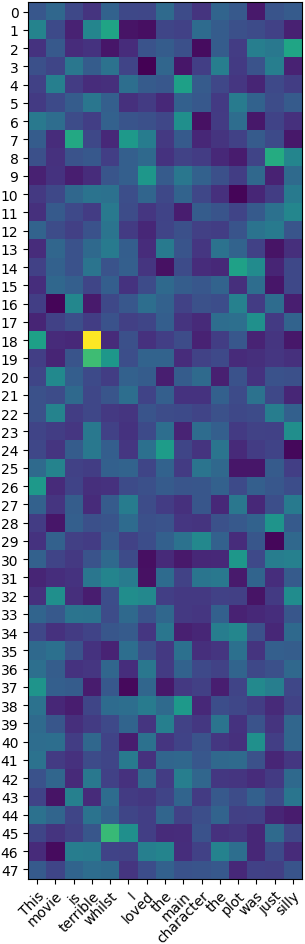
\includegraphics[height=0.6\textheight]{imgs/example_1.png}
        \caption{Prediction: strongly negative}
    \end{subfigure}
    \hspace{.05\textwidth}
    \begin{subfigure}{.55\textwidth}
        \centering
        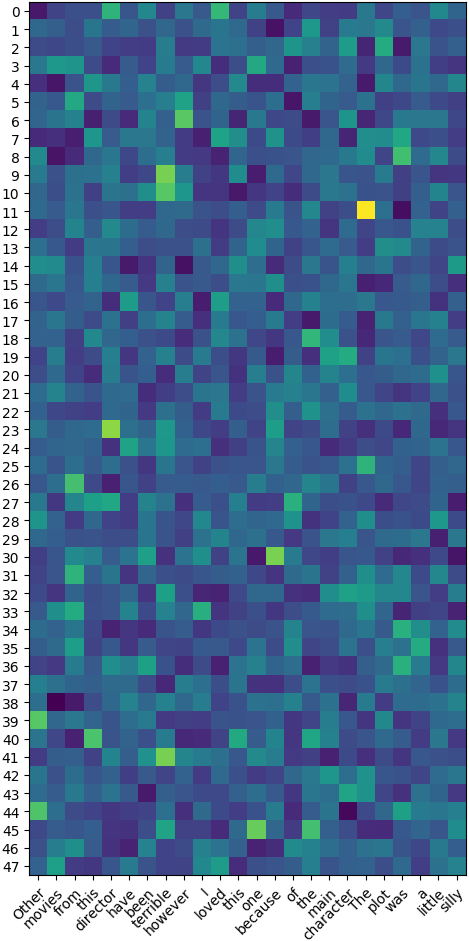
\includegraphics[height=0.6\textheight]{imgs/example_2.png}
        \caption{Prediction: weakly positive}
    \end{subfigure}
    \caption{The attention weights across all 48 heads with predicted classification for the single layer IMDb token level text classification Transformer model on two unseen and similar examples.}
    \label{fig:wide_attention_full}
\end{figure}

Figure \ref{fig:wide_attention_full} shows the attention scores for every head for our example in \Cref{sec:disscusion:interp}.


\section{Small Model Ablation Study}\label{appendix:ablation}

In order to verify the validity of going wide \textbf{and} going shallow, we run 'small' vanilla attention Transformer models on all 4 tasks.
These models use the same number of heads per layer as the deepest models but have only 1 layer.
Therefore 8 heads on both IMDb tasks and Listops, and 4 heads on the document matching task.
These results are given in \cref{table:smol} along with repeats of the averages from the deepest and widest Transformer models.
As we can see the small model always performs worse than at least the widest one, though surprisingly beating the deep model on the Listops task.
On the IMDb and document matching tasks it consistently performs 1.5\%-3\% worse than the others, as expected.

\begin{table}[!h]
    \caption{Test accuracy for each task for the small vanilla Transformer model compared to its fully wide and fully deep counterparts.}
    \label{table:smol}
    \begin{center}
        \begin{tabular}{l | l l l}
            \toprule
            {\bf Task} & \textbf{Deepest} & \textbf{Widest} & \textbf{Small} \\
            \midrule
            IMDb Token Level & 85.8 & 85.5 & 84.0 \\
            IMDb Byte Level & 62.6 & 62.4 & 59.6 \\
            Listops & 35.7 & 37.2 & 36.9 \\
            Document Matching & 64.0 & 64.4 & 62.4 \\
            \bottomrule
        \end{tabular}
    \end{center}
\end{table}

